\documentclass[aspectratio=169]{beamer}
\usetheme{Madrid}
\usecolortheme{default}
% Packages
\usepackage{amsmath}
\usepackage{amssymb}
\usepackage{graphicx}
\usepackage{booktabs}
\usepackage{algorithm}
\usepackage{algorithmic}
% Title Information
\title{Unsupervised Image Segmentation and Denoising}
\date{}

\begin{document}
% Title Slide
\begin{frame}
\titlepage
\end{frame}
% Outline
\begin{frame}{Outline}
\tableofcontents
\end{frame}
% ==================== SECTION 1: INTRODUCTION ====================
\section{Introduction}
\begin{frame}{The Problem: Unsupervised Segmentation}
\begin{block}{Definition}
The task of partitioning an image into semantically meaningful regions (objects vs. background) \textbf{without} using any pixel-level annotations during training.
\end{block}
\vspace{0.5cm}
\textbf{The Challenge:}
\begin{itemize}
    \item Without labels, models must rely on intrinsic image properties
    \item Color, texture, edges or self-supervised features
    \item Must discover objects autonomously
\end{itemize}
\end{frame}
\begin{frame}{Why Unsupervised Segmentation?}
\begin{columns}
\begin{column}{0.5\textwidth}
\textbf{Scalability}
\begin{itemize}
    \item Manual pixel-wise annotation is expensive
    \item Time-consuming for large datasets
\end{itemize}
\vspace{0.3cm}
\textbf{Generalization}
\begin{itemize}
    \item Not restricted to predefined classes
    \item Can discover novel object categories
\end{itemize}
\end{column}
\begin{column}{0.5\textwidth}
\textbf{Discovery}
\begin{itemize}
    \item Useful for exploring unlabeled data
    \item Enables zero-shot segmentation
\end{itemize}
\vspace{0.3cm}
% Placeholder for image
\begin{center}
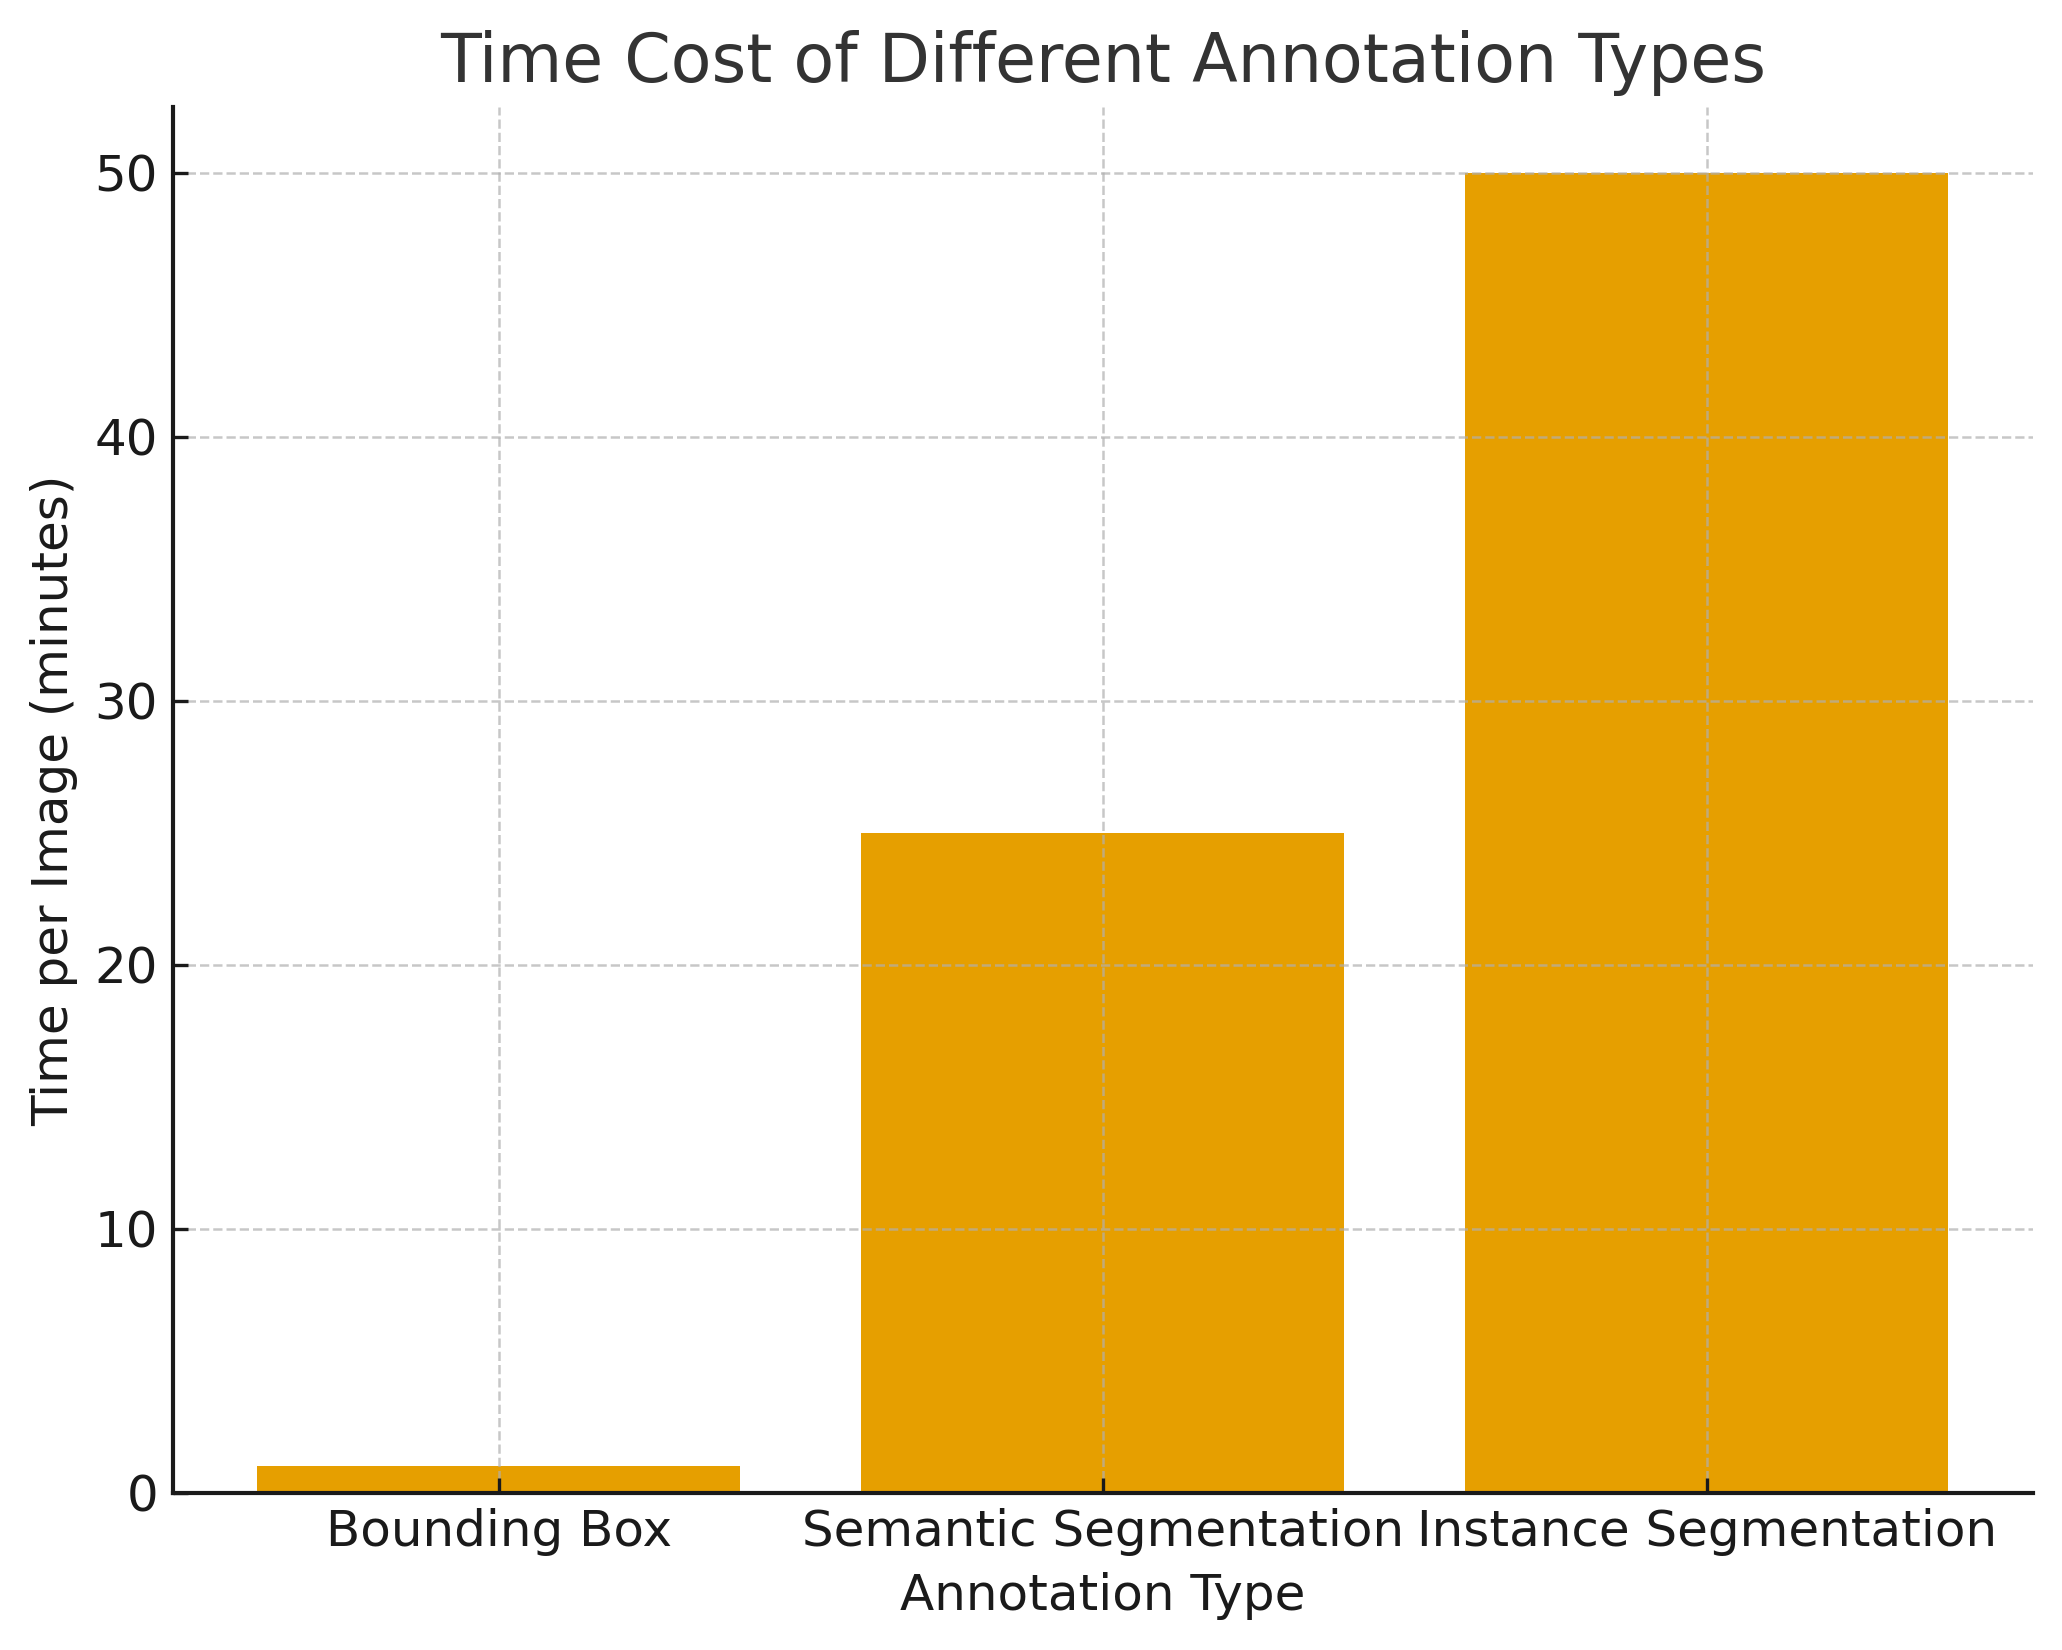
\includegraphics[width=0.7\textwidth]{figure1.png}
\end{center}
\end{column}
\end{columns}
\end{frame}
\begin{frame}{Project Scope}
\begin{block}{Binary Segmentation Focus}
Distinguishing between:
\begin{itemize}
    \item \textbf{"Things" (Foreground):} Countable objects (person, car, bird)
    \item \textbf{"Stuff" (Background):} Amorphous regions (sky, grass, road)
\end{itemize}
\end{block}
\vspace{0.5cm}
\textbf{Project Objectives:}
\begin{enumerate}
    \item Implement \textbf{TokenCut}: Training-free, graph-based method
    \item Implement \textbf{EAGLE}: Self-supervised contrastive learning
    \item Compare on COCO-Stuff-27 dataset
    \item Analyze accuracy vs. efficiency trade-offs
\end{enumerate}
\end{frame}
% ==================== SECTION 2: RELATED WORK ====================
\section{Related Work}
\begin{frame}{Traditional Methods}
\begin{block}{Graph-Based Segmentation}
\textbf{Normalized Cuts (Shi \& Malik, 2000)}
\begin{itemize}
    \item Treats segmentation as graph partitioning
    \item Pixels = nodes, edges = similarity
    \item Minimize cut cost while maximizing internal association
    \item \textit{Limitation:} Relies on low-level features (RGB, gradients)
\end{itemize}
\end{block}
\vspace{0.3cm}
\begin{block}{Clustering Methods}
\textbf{K-Means / Mean Shift}
\begin{itemize}
    \item Clusters pixels in color space
    \item \textit{Limitation:} No semantic understanding; over-segments textured objects
\end{itemize}
\end{block}
\end{frame}

\begin{frame}{Graph Based Segmentation Example}
\begin{center}
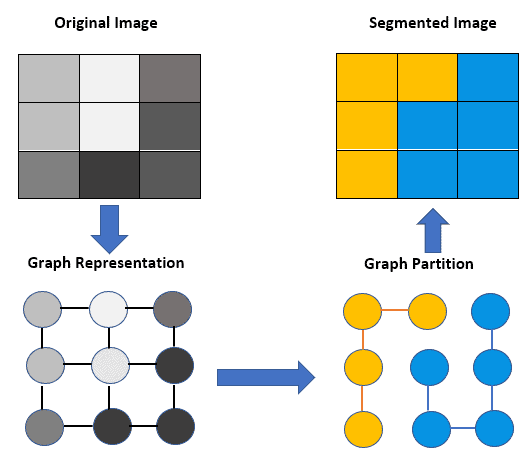
\includegraphics[width=0.5\textwidth]{graph.png}
\end{center}
\end{frame}


\begin{frame}{Deep Learning Era}
\textbf{Supervised Learning}
\begin{itemize}
    \item FCN, U-Net, DeepLab achieve SOTA results
    \item Require massive annotated datasets
\end{itemize}
\vspace{0.5cm}
\textbf{Self-Supervised Learning (SSL)}
\begin{itemize}
    \item \textbf{Contrastive Learning:} SimCLR, MoCo
    \item \textbf{Vision Transformers \& DINO:}
    \begin{itemize}
        \item DINO = Distillation with No Labels
        \item Self-attention maps highlight salient objects
        \item \textcolor{blue}{Both TokenCut and EAGLE build on DINO features}
    \end{itemize}
\end{itemize}
\vspace{0.3cm}
\begin{center}
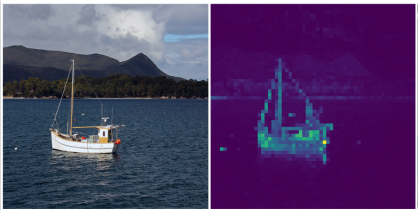
\includegraphics[width=0.3\textwidth]{figure2.png}
\end{center}
\end{frame}
% ==================== SECTION 3: TOKENCUT ====================
\section{TokenCut Methodology}
\begin{frame}{TokenCut: Overview}
\begin{block}{Core Concept}
"Segmenting Objects without Training" - Leverages DINO features + Normalized Cuts
\end{block}
\textbf{Workflow:}
\begin{enumerate}
    \item Extract features from pre-trained DINO model
    \item Construct graph where nodes = image patches
    \item Solve spectral clustering to find object
\end{enumerate}
\vspace{0.3cm}
\begin{figure}
\centering
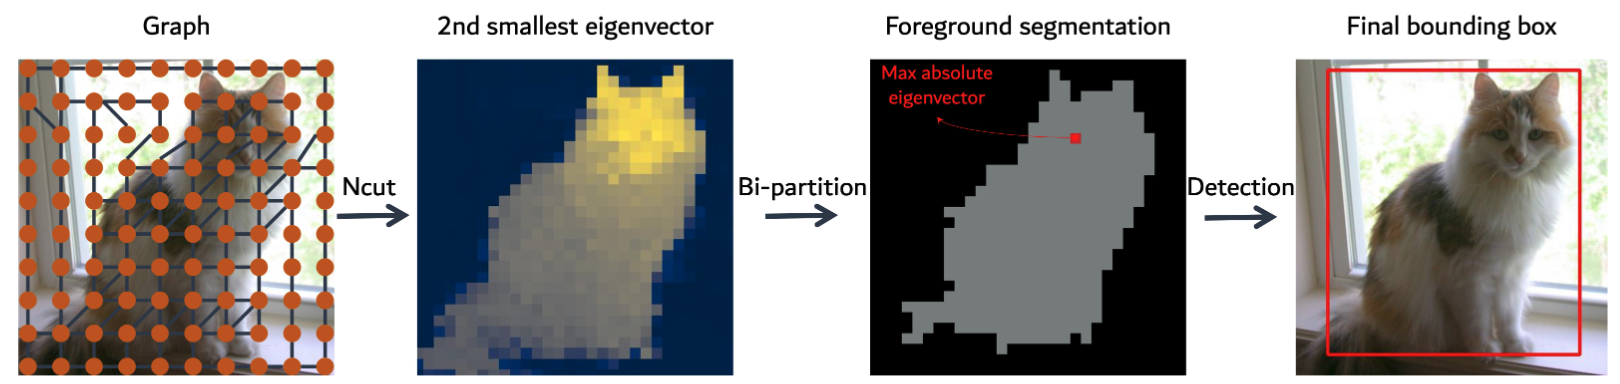
\includegraphics[width=0.8\textwidth]{figure3.png}
\end{figure}
\end{frame}
\begin{frame}{TokenCut: Feature Extraction}
\textbf{DINO ViT-Small}
\begin{itemize}
    \item Vision Transformer pre-trained with DINO
    \item \textbf{Input:} Image $I \in \mathbb{R}^{H \times W \times 3}$
    \item \textbf{Patches:} Split into $16 \times 16$ patches
    \item \textbf{Features:} $F \in \mathbb{R}^{N \times D}$
    \begin{itemize}
        \item $N$ = number of patches
        \item $D$ = feature dimension
    \end{itemize}
\end{itemize}
\vspace{0.5cm}
\begin{alertblock}{Why DINO?}
DINO features exhibit \textbf{semantic consistency}. Patches from the same object (e.g., dog head + tail) have high cosine similarity, even if RGB values differ.
\end{alertblock}
\end{frame}
\begin{frame}{TokenCut: Graph Construction}
\textbf{Similarity Graph} $G = (V, E)$
\begin{itemize}
    \item \textbf{Nodes ($V$):} The $N$ image patches
    \item \textbf{Edges ($E$):} Weighted by similarity
\end{itemize}
\vspace{0.5cm}
\textbf{Affinity Matrix ($A$):}
\begin{equation}
A_{ij} = \begin{cases} 
\cos(f_i, f_j) & \text{if } \cos(f_i, f_j) > \tau \\
0 & \text{otherwise}
\end{cases}
\end{equation}
\begin{itemize}
    \item $\tau$: Threshold to remove weak connections
    \item Captures \textbf{semantic relationship} between patch pairs
\end{itemize}
\end{frame}
\begin{frame}{TokenCut: Normalized Cut Problem}
\textbf{Objective:} Partition vertices $V$ into disjoint sets $A$ (Foreground) and $B$ (Background)
\begin{equation}
\text{Ncut}(A, B) = \frac{\text{cut}(A, B)}{\text{assoc}(A, V)} + \frac{\text{cut}(A, B)}{\text{assoc}(B, V)}
\end{equation}
Where:
\begin{itemize}
    \item $\text{cut}(A, B) = \sum_{i \in A, j \in B} w_{ij}$ (sum of edge weights crossing the cut)
    \item $\text{assoc}(A, V) = \sum_{i \in A} d_i$ (total connection from $A$ to all nodes)
\end{itemize}
\vspace{0.3cm}
\begin{block}{Intuition}
Cut \textit{weak} edges (low similarity) such that remaining partitions are \textit{strongly} connected internally.
\end{block}
\end{frame}
\begin{frame}{TokenCut: Solving the N-Cut}
\textbf{Spectral Relaxation} (NP-hard $\rightarrow$ Eigenvalue problem):
\begin{equation}
D^{-\frac{1}{2}} (D - A) D^{-\frac{1}{2}} z = \lambda z
\end{equation}
\begin{itemize}
    \item $D$: Degree matrix (diagonal, $D_{ii} = \sum_j A_{ij}$)
    \item $L = D - A$: Laplacian matrix
    \item $\mathcal{L}_{sym} = D^{-\frac{1}{2}} L D^{-\frac{1}{2}}$: Normalized Laplacian
\end{itemize}
\vspace{0.5cm}
\begin{alertblock}{Solution}
The \textbf{second smallest eigenvector} (Fiedler vector) of $\mathcal{L}_{sym}$ provides the optimal real-valued bipartition. Threshold at mean or 0 to get binary mask.
\end{alertblock}
\end{frame}
\begin{frame}{TokenCut: Algorithm Summary}
\begin{algorithm}[H]
\caption{TokenCut}
\begin{algorithmic}[1]
\STATE \textbf{Input:} Image $I$
\STATE Extract features $F$ using DINO ViT-S/16
\STATE Compute affinity $A = F F^\top$ (cosine similarity)
\STATE Compute degree matrix $D$ and $\mathcal{L}_{sym}$
\STATE Solve $\mathcal{L}_{sym} z = \lambda z$ for 2nd smallest eigenvector $y$
\STATE Threshold $y$ to obtain binary mask $M$
\STATE \textbf{Optional:} Refine with bilateral solver or CRF
\STATE \textbf{Output:} Segmentation mask $M$
\end{algorithmic}
\end{algorithm}

\end{frame}

\begin{frame}{TokenCut Evaluation Datasets}
\begin{columns}
\begin{column}{0.5\textwidth}
\begin{block}{ECSSD Dataset}
\textbf{Extended Complex Scene Saliency}
\end{block}
\begin{itemize}
    \item \textbf{Size:} 1,000 images
    \item \textbf{Content:} Natural scenes with prominent objects
    \item \textbf{Annotations:} Pixel-wise binary masks
\end{itemize}
\vspace{0.2cm}
\textbf{Characteristics:}
\begin{itemize}
    \item Clear figure-ground separation
    \item Centered salient objects
    \item Varying complexity levels
\end{itemize}

\end{column}

\begin{column}{0.5\textwidth}
\begin{block}{CUB-200-2011 Dataset}
\textbf{Caltech-UCSD Birds}
\end{block}
\begin{itemize}
    \item \textbf{Size:} 11,788 images
    \item \textbf{Classes:} 200 bird species
    \item \textbf{Annotations:} Segmentation masks + keypoints
\end{itemize}
\vspace{0.2cm}
\textbf{Challenges:}
\begin{itemize}
    \item Complex feather textures
    \item Thin structures (legs, beaks)
    \item Multi-colored plumage
\end{itemize}

\end{column}
\end{columns}
\end{frame}

% ==================== TOKENCUT QUALITATIVE RESULTS ====================
\begin{frame}{TokenCut: Qualitative Results}


\begin{columns}
\begin{column}{0.5\textwidth}
\begin{center}
\textbf{ECSSD Dataset}
\end{center}
\begin{center}
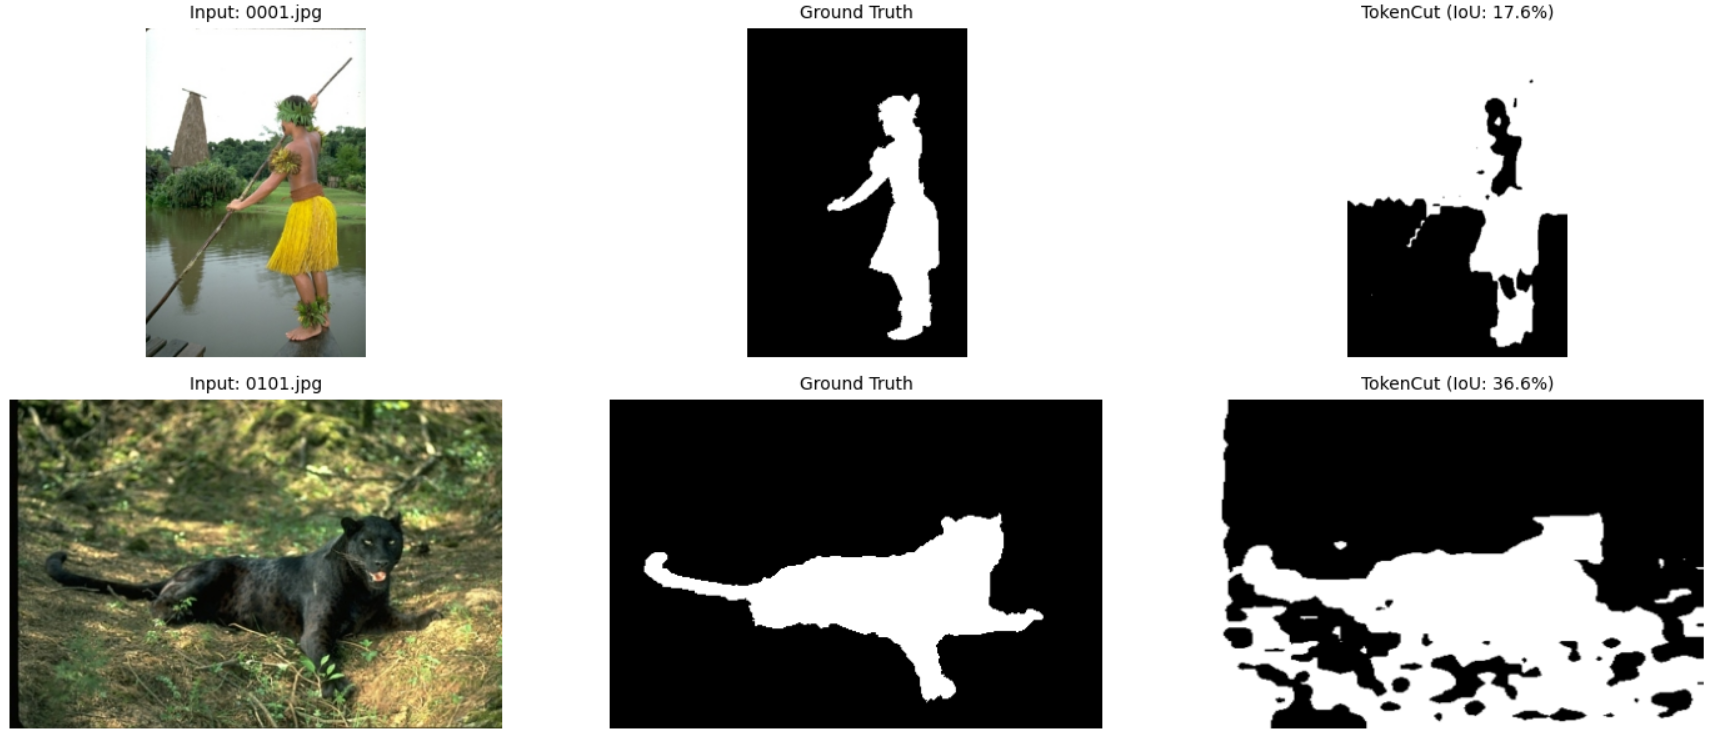
\includegraphics[width=0.95\textwidth]{tokencut_ecssd.png}
\end{center}

\end{column}

\begin{column}{0.5\textwidth}
\begin{center}
\textbf{CUB-200-2011 Dataset}
\end{center}
\begin{center}
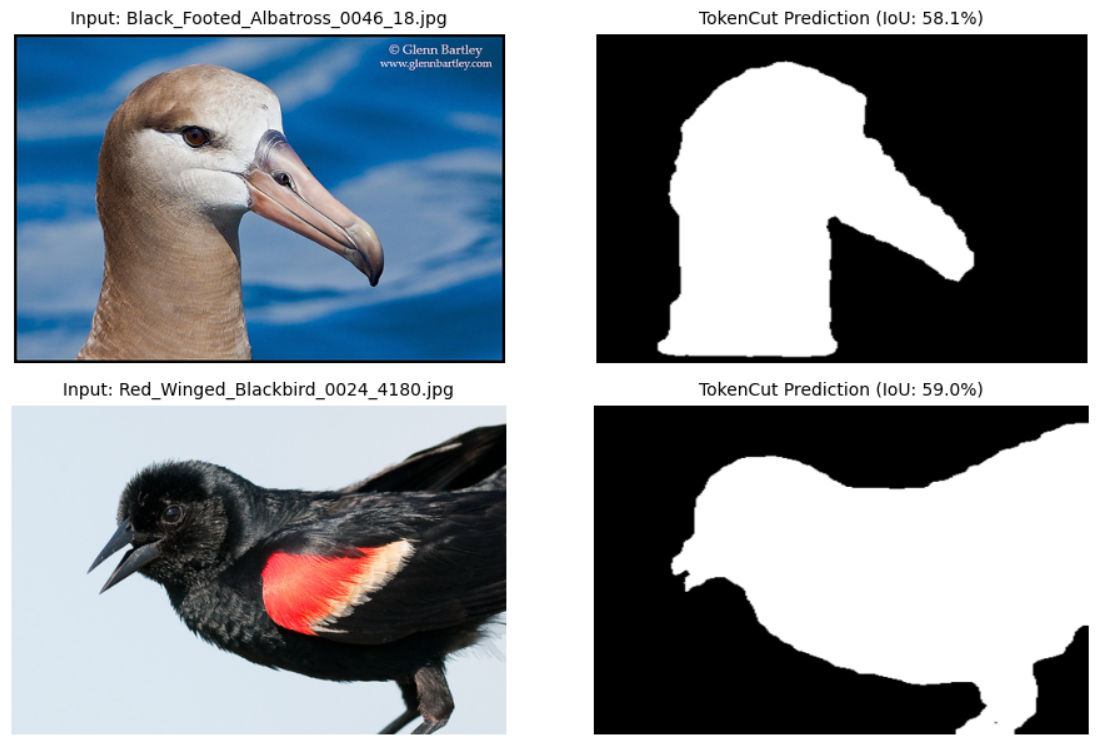
\includegraphics[width=0.95\textwidth]{tokencut_cub.png}
\end{center}

\end{column}
\end{columns}
\end{frame}

% ==================== TOKENCUT QUANTITATIVE RESULTS ====================
\begin{frame}{TokenCut: Quantitative Analysis}
\begin{columns}
\begin{column}{0.5\textwidth}
\begin{table}
\centering
\begin{tabular}{lcc}
\toprule
\textbf{Dataset} & \textbf{mIoU} \\
\midrule
ECSSD & \textbf{42.82\%} \\
CUB-200 & 32.97\% \\
COCO-Stuff-27 & 31.75\%  \\
\bottomrule
\end{tabular}
\caption{TokenCut Performance}
\end{table}


\end{column}

\begin{column}{0.5\textwidth}
\textbf{Performance Analysis:}

\begin{block}{Strong Performance (ECSSD)}
\begin{itemize}
    \item High-contrast objects
    \item DINO features align well
\end{itemize}
\end{block}



\begin{alertblock}{Limitations}
\begin{itemize}
    \item \textbf{Color sensitivity:} Fragments multi-colored objects
    \item \textbf{Graph-cut bias:} Prefers single dominant object
\end{itemize}
\end{alertblock}
\end{column}
\end{columns}
\end{frame}

% ==================== SECTION 4: EAGLE ====================
\section{EAGLE Methodology}
\begin{frame}{EAGLE: Overview}
\begin{block}{Eigen Aggregation Learning}
Addresses the \textbf{"Chicken-and-Egg"} problem:
\begin{itemize}
    \item Good segmentation needs good features
    \item Good features need good segmentation
\end{itemize}
\end{block}
\textbf{Solution:} Iterative refinement
\begin{enumerate}
    \item Use spectral priors (\textbf{EiCue}) to initialize masks
    \item Use contrastive learning (\textbf{ObjNCELoss}) to refine features
\end{enumerate}

\end{frame}

\begin{frame}{EAGLE: Overview}

\begin{center}
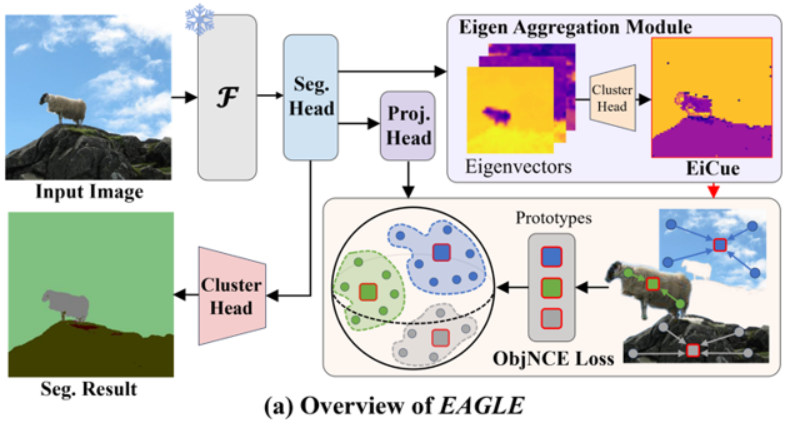
\includegraphics[width=0.8\textwidth]{eagle_train_pipeline.png}
\end{center}
\end{frame}

\begin{frame}{EAGLE: Architecture}
\textbf{Pipeline Components:}
\begin{enumerate}
    \item \textbf{Backbone:} DINO ViT extracts features
    \item \textbf{EiCue Module:} Generates pseudo-masks via spectral clustering
    \item \textbf{Projection Head:} Maps features to embedding space
    \item \textbf{Training:}
    \begin{itemize}
        \item \textit{Linear Probe:} Predicts class labels (supervised by pseudo-masks)
        \item \textit{Cluster Probe:} Predicts cluster assignments (unsupervised)
        \item \textit{ObjNCELoss:} Refines feature space
    \end{itemize}
\end{enumerate}
\end{frame}

\begin{frame}{EAGLE: Architecture}

\begin{center}
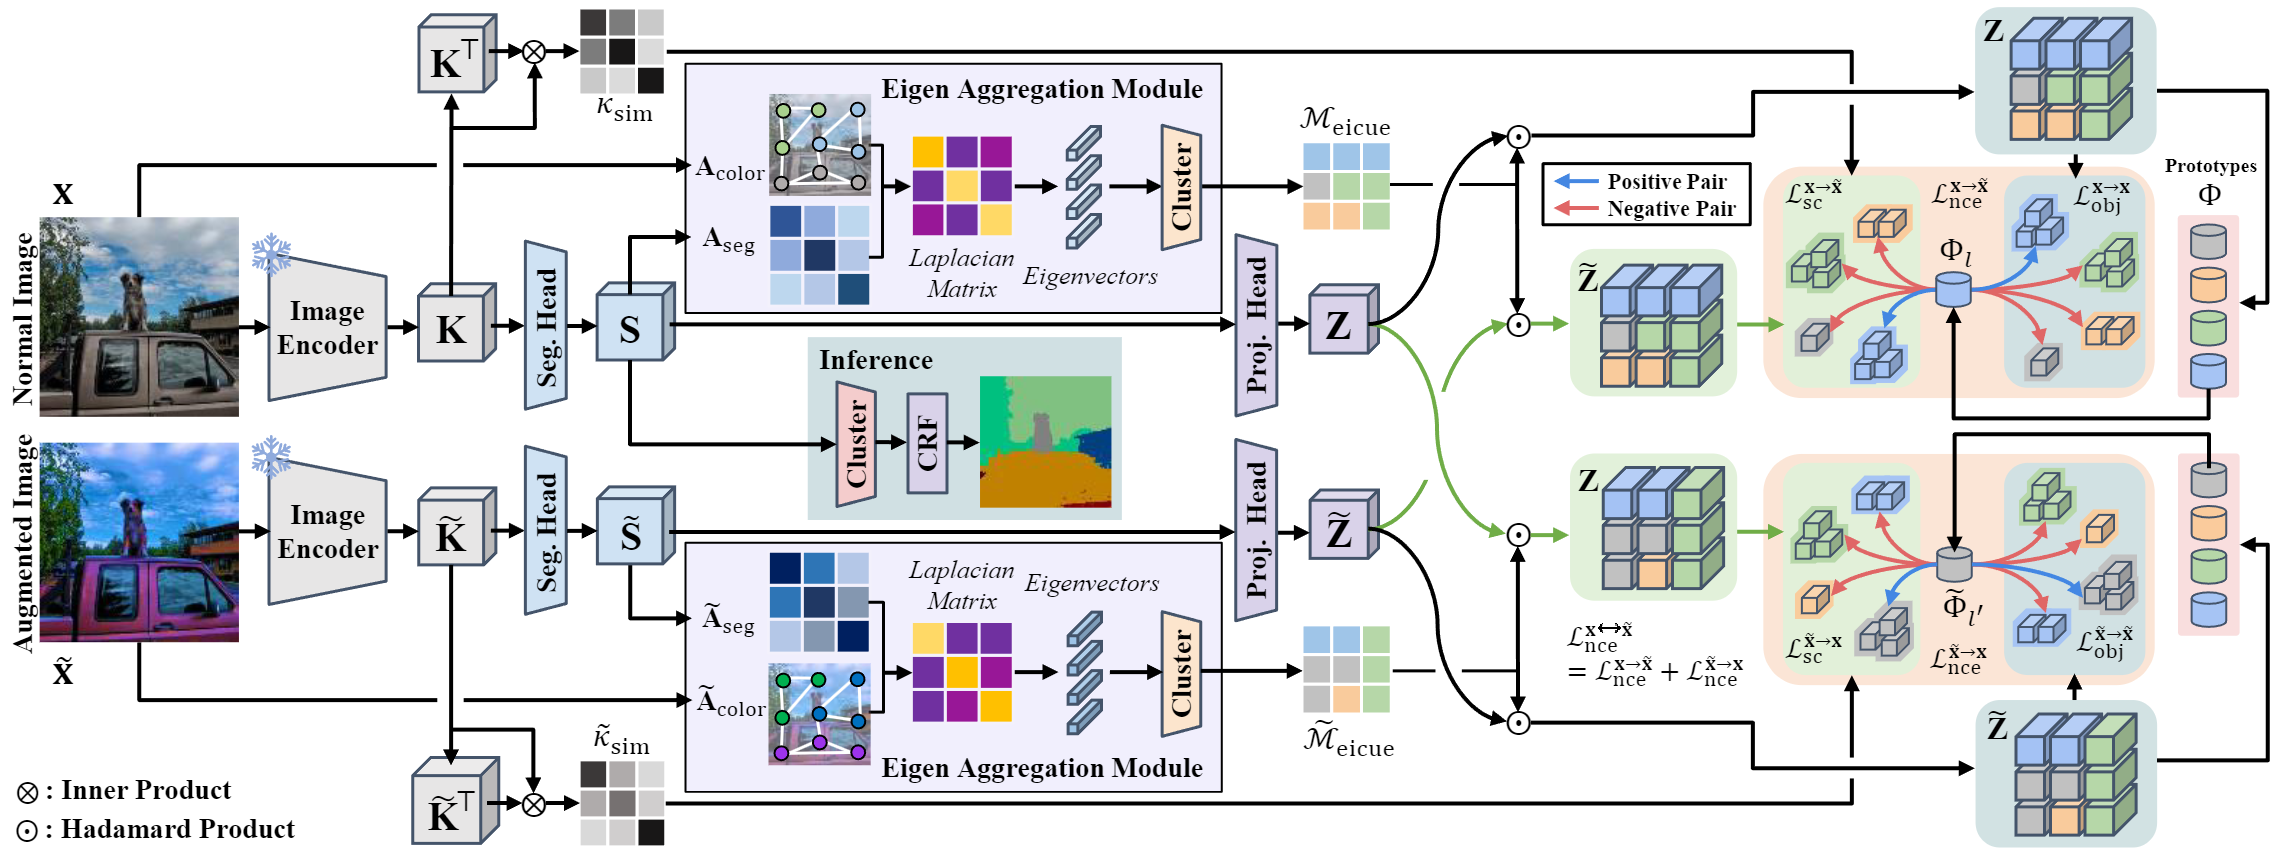
\includegraphics[width=0.8\textwidth]{eagle_architecture.png}
\end{center}
\end{frame}


\begin{frame}{EAGLE: EiCue (Eigen Aggregation)}
\textbf{Improving Spectral Clustering}
Standard K-means on features is noisy. EAGLE uses \textbf{spectral clustering} on the Laplacian.
\vspace{0.5cm}
\textbf{Affinity Construction:}
\begin{equation}
A = A_{color} + A_{seg}
\end{equation}
\begin{itemize}
    \item $A_{color}$: Local RGB differences (captures boundaries)
    \item $A_{seg} = S S^\top$: Feature dot products (captures semantics)
    \item $S$: Learnable semantic features
\end{itemize}
\vspace{0.3cm}
\textbf{Spectral Decomposition:}
\begin{itemize}
    \item Compute eigenvectors of Laplacian of $A$
    \item Run K-means on \textit{eigenvectors}, not raw features
    \item \textbf{Result:} Coherent object masks
\end{itemize}
\end{frame}
\begin{frame}{EAGLE: K-means vs. EiCue}
\begin{center}
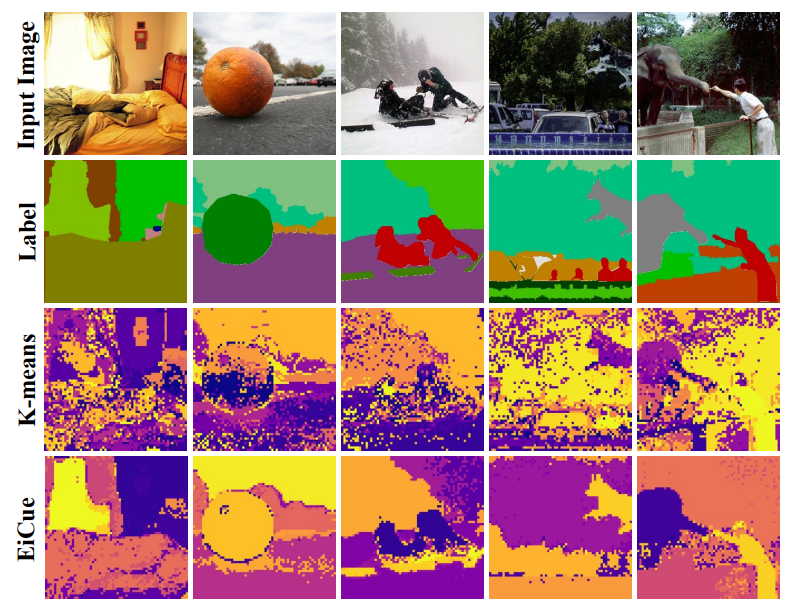
\includegraphics[width=0.4\textwidth]{kmean-eicue.png}
\end{center}
\vspace{0.3cm}
\textbf{Observation:}
\begin{itemize}
    \item \textbf{K-means:} Fragments objects based on texture/color
    \item \textbf{EiCue:} Groups semantically related regions (e.g., entire bed)
\end{itemize}
\end{frame}
\begin{frame}{EAGLE: ObjNCELoss (Concept)}
\textbf{Object-Centric Contrastive Learning}
Standard InfoNCE works on \textit{images} or \textit{pixels}. EAGLE extends to \textit{objects}.
\vspace{0.5cm}
\begin{itemize}
    \item \textbf{Positive Pairs:} Pixel feature + prototype (centroid) of its object
    \item \textbf{Negative Pairs:} Pixel feature + prototypes of \textit{other} objects
\end{itemize}
\vspace{0.3cm}
\begin{block}{Goal}
Pull pixels towards their object center, push away from other objects.
\end{block}
\end{frame}
\begin{frame}{EAGLE: ObjNCELoss (Math)}
\begin{equation}
\mathcal{L}_{ObjNCE} = - \sum_{i \in \Omega} \log \frac{\exp(f_i \cdot c_{y_i} / \tau)}{\sum_{j=1}^{K} \exp(f_i \cdot c_j / \tau)}
\end{equation}
\textbf{Notation:}
\begin{itemize}
    \item $f_i$: Feature vector of pixel $i$
    \item $c_{y_i}$: Prototype vector of class $y_i$ (assigned to pixel $i$)
    \item $c_j$: Prototype vector of class $j$
    \item $K$: Number of clusters/classes
    \item $\tau$: Temperature scaling parameter
\end{itemize}
\vspace{0.3cm}
\textbf{Effect:} Refines feature space, making "thing" and "stuff" classes distinct.
\end{frame}
% ==================== SECTION 5: EXPERIMENTS ====================
\section{Experimental Setup}
\begin{frame}{Dataset: COCO-Stuff-27}
\begin{columns}
\begin{column}{0.5\textwidth}
\begin{block}{Overview}
\begin{itemize}
    \item Curated subset of COCO-Stuff-164K
    \item 27 super-categories for semantic segmentation
    \item 15 "Thing" classes (countable objects)
    \item 12 "Stuff" classes (amorphous regions)
\end{itemize}
\end{block}

\textbf{Thing Classes (Examples):}
\begin{itemize}
    \item Person, vehicle, animal
    \item Furniture, appliances
    \item Sports equipment
\end{itemize}
\end{column}

\begin{column}{0.5\textwidth}
\textbf{Stuff Classes (Examples):}
\begin{itemize}
    \item Sky, grass, water, road
    \item Wall, building, floor
    \item Tree, sand, snow
\end{itemize}

\vspace{0.3cm}
\begin{block}{Binary Task}
\begin{itemize}
    \item \textbf{Foreground:} All "Thing" objects
    \item \textbf{Background:} All "Stuff" regions
    \item Primary benchmark for evaluating thing/stuff separation
\end{itemize}
\end{block}

\textbf{Dataset Statistics:}
\begin{itemize}
    \item Complex real-world scenes
    \item Multiple objects per image
    \item Rich contextual information
\end{itemize}
\end{column}
\end{columns}
\end{frame}
\begin{frame}{Evaluation Metrics}
\textbf{1. Mean Intersection over Union (mIoU)}
\begin{equation}
\text{IoU} = \frac{\text{Area of Overlap}}{\text{Area of Union}} = \frac{TP}{TP + FP + FN}
\end{equation}
\begin{itemize}
    \item Standard metric for segmentation accuracy
    \item Report mIoU for binary case (Foreground/Background)
\end{itemize}
\vspace{0.5cm}
\textbf{2. Pixel Accuracy}
\begin{equation}
\text{Accuracy} = \frac{TP + TN}{TP + TN + FP + FN}
\end{equation}
\begin{itemize}
    \item Ratio of correctly classified pixels
\end{itemize}
\end{frame}
% ==================== SECTION 6: RESULTS ====================
\section{Results \& Evaluation}
\begin{frame}{EAGLE: Quantitative Results}
\begin{table}
\centering
\begin{tabular}{lcc}
\toprule
\textbf{Probe Type} & \textbf{mIoU} & \textbf{Accuracy} \\
\midrule
Linear Probe & \textbf{41.19\%} & \textbf{68.65\%} \\
Cluster Probe & 24.40\% & 50.79\% \\
Binary (Thing/Stuff) & \textbf{62.03\%} & - \\
\bottomrule
\end{tabular}
\caption{COCO-Stuff-27 Performance}
\end{table}
\vspace{0.3cm}
\textbf{Observations:}
\begin{itemize}
    \item Binary mIoU (62.03\%) significantly higher than TokenCut
    \item Linear Probe outperforms Cluster Probe
    \item EiCue effectively groups semantic parts
\end{itemize}
\end{frame}
\begin{frame}{EAGLE: Qualitative Results}
\begin{center}
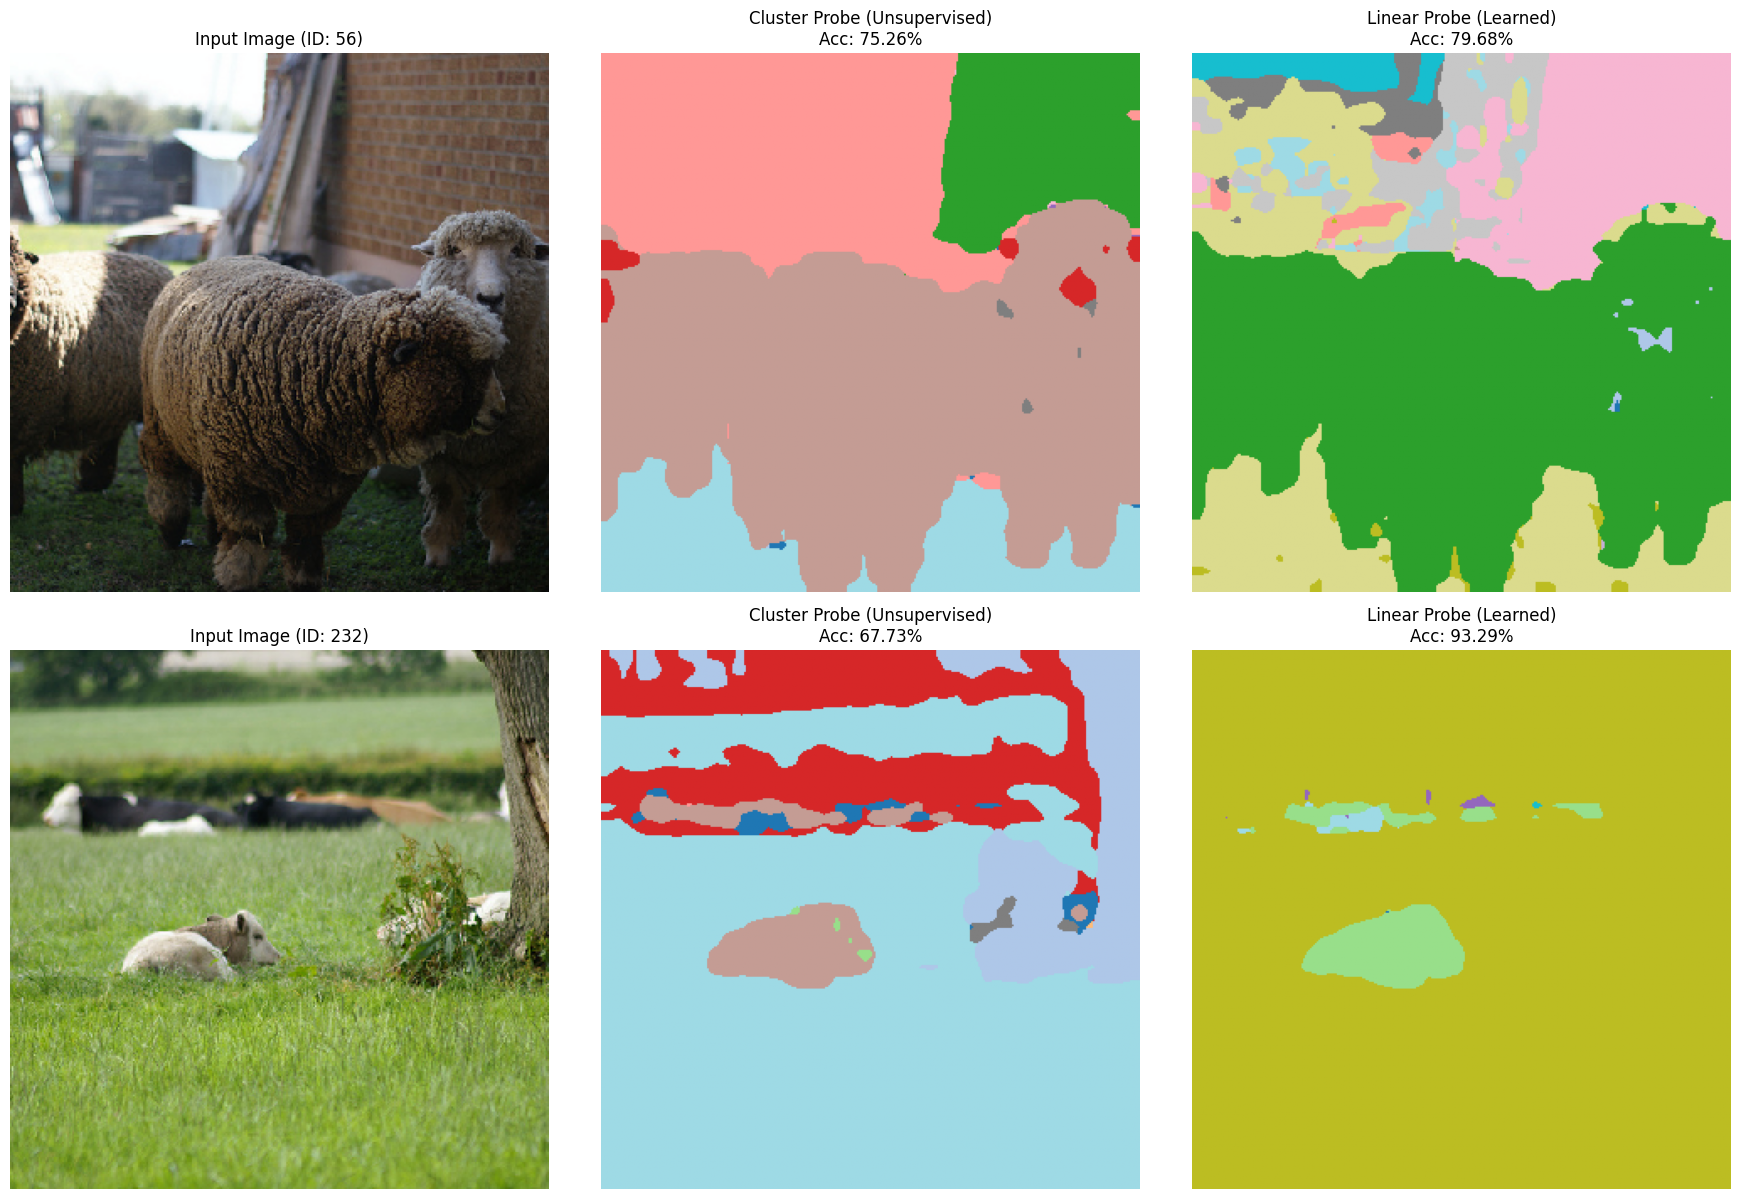
\includegraphics[width=0.7\textwidth]{eagle-res.png}
\end{center}
\end{frame}
\begin{frame}{TokenCut vs Eagle: Differences}
\begin{table}
\centering
\small
\begin{tabular}{p{0.25\textwidth} p{0.35\textwidth} p{0.35\textwidth}}
\toprule
\textbf{Aspect} & \textbf{TokenCut} & \textbf{EAGLE} \\
\midrule
\textbf{Core Approach} & Graph-based (Normalized Cuts) & Contrastive Learning (ObjNCELoss) \\
\addlinespace
\textbf{Training} & \textbf{Training-free} (Inference only) & \textbf{Self-Supervised} (Requires training) \\
\addlinespace
\textbf{Optimization} & Per-image spectral clustering & Learned weights (Feed-forward) \\
\addlinespace
\textbf{Inference Speed} & Slow ($\sim$1.5s) - Solve Eigenproblem & Fast ($\sim$0.13s) - Linear projection \\
\addlinespace
\textbf{Segmentation} & Binary (Foreground/Background) & Semantic (Multi-class capable) \\
\addlinespace
\textbf{Resolution} & High (Patch-level graph) & Low (Feature-level maps) \\
\bottomrule
\end{tabular}
\end{table}

\vspace{0.1cm}

\begin{alertblock}{Fundamental Difference}
TokenCut treats segmentation as a \textbf{mathematical optimization problem} on a graph for each image individually. EAGLE treats it as a \textbf{representation learning problem}, learning to recognize objects across the entire dataset.
\end{alertblock}
\end{frame}


\begin{frame}{TokenCut vs Eagle: Qualitative Comparison (COCO Stuff)}
\begin{center}
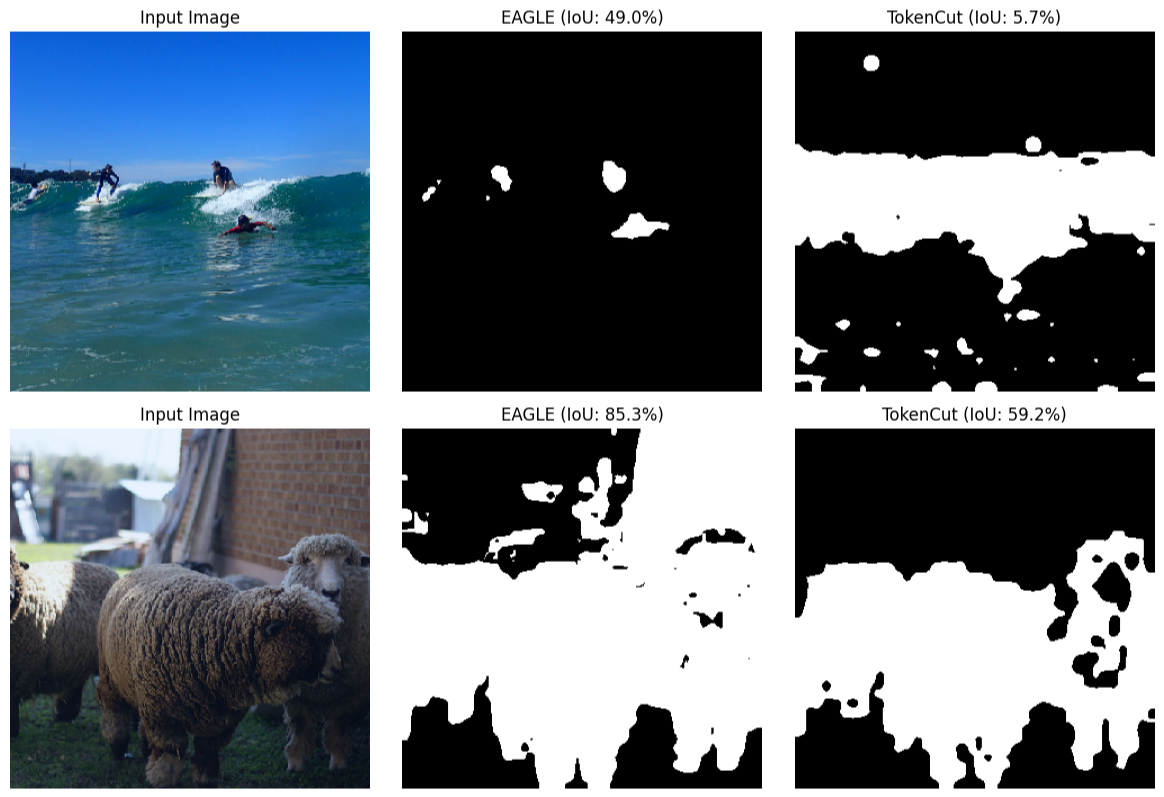
\includegraphics[width=0.7\textwidth]{eagle-token-coco.png}
\end{center}

\end{frame}

\begin{frame}{TokenCut vs Eagle: Qualitative Comparison (Real Images)}
\begin{center}
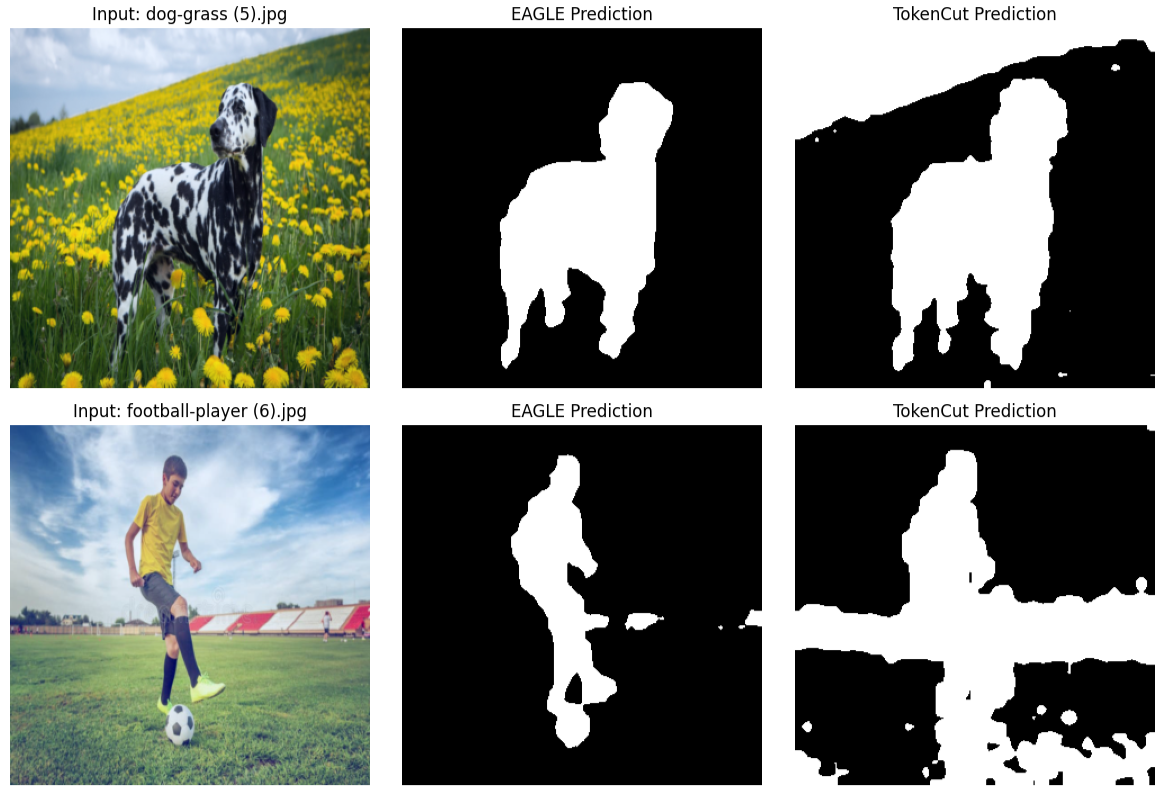
\includegraphics[width=0.7\textwidth]{eagle-token-real.png}
\end{center}

\end{frame}

% ==================== SECTION 7: COMPARATIVE ANALYSIS ====================
\section{Comparative Analysis}
\begin{frame}{Performance Comparison}
\begin{table}
\centering
\begin{tabular}{lcc}
\toprule
\textbf{Feature} & \textbf{TokenCut} & \textbf{EAGLE} \\
\midrule
Approach & Graph-based (N-Cut) & Contrastive Learning \\
Training & None & Required (SSL) \\
Binary mIoU & 31.75\% & \textbf{62.03\%} \\
Resolution & High (Pixel-level) & Low (Feature-level) \\
Robustness & Low (Color-sensitive) & High (Semantic) \\
\bottomrule
\end{tabular}
\end{table}
\vspace{0.5cm}
\begin{alertblock}{Verdict}
EAGLE is superior for semantic segmentation accuracy (+30\% mIoU).
\end{alertblock}
\end{frame}
\begin{frame}{Computational Efficiency}
\begin{table}
\centering
\begin{tabular}{lcc}
\toprule
\textbf{Model} & \textbf{Time/Image} & \textbf{Bottleneck} \\
\midrule
TokenCut & $\sim$1.50 sec & Eigendecomposition ($O(N^3)$) \\
EAGLE & \textbf{$\sim$0.13 sec} & Feed-forward pass ($O(N)$) \\
\bottomrule
\end{tabular}
\end{table}
\vspace{0.5cm}
\textbf{Scalability:}
\begin{itemize}
    \item \textbf{TokenCut:} $O(N^3)$ complexity - hard to scale to high-res
    \item \textbf{EAGLE:} $O(N)$ complexity - suitable for real-time
\end{itemize}
\vspace{0.3cm}
\begin{block}{Verdict}
EAGLE is suitable for real-time applications; TokenCut limited to offline processing.
\end{block}
\end{frame}
% ==================== SECTION 8: CONCLUSION ====================
\section{Conclusion \& Future Work}
\begin{frame}{Conclusion}
\textbf{Summary of Findings:}
\begin{enumerate}
    \item EAGLE outperforms TokenCut by \textbf{+30\% mIoU} on complex binary segmentation
    \item \textbf{Spectral Initialization (EiCue)} is critical for avoiding local optima
    \item \textbf{Contrastive Learning (ObjNCELoss)} refines features for object-centric representations
    \item \textbf{Training-free vs. Learned:} While TokenCut is attractive for zero-shot, EAGLE's learned representations provide robustness
\end{enumerate}
\end{frame}
\begin{frame}{Future Work}
\textbf{1. Integration with Diffusion Models}
\begin{itemize}
    \item Leverage Stable Diffusion features (ODISE) for boundary precision
    \item Address EAGLE's low-resolution limitation
\end{itemize}
\vspace{0.3cm}
\textbf{2. Multi-Scale Processing}
\begin{itemize}
    \item Combine TokenCut's edge sensitivity with EAGLE's semantic coherence
    \item Hybrid model for best of both worlds
\end{itemize}
\vspace{0.3cm}
\textbf{3. Video Segmentation}
\begin{itemize}
    \item Extend EAGLE to video with temporal consistency loss
    \item Enforce consistent object IDs across frames
\end{itemize}
\end{frame}
% ==================== SECTION 9: REFERENCES ====================
\section{References}
\begin{frame}{References}
\begin{thebibliography}{9}
\bibitem{tokencut} Wang, Y., et al. (2022). \textit{Self-Supervised Transformers for Unsupervised Object Discovery using Normalized Cut.} CVPR 2022.
\bibitem{eagle} \textit{Eigen Aggregation Learning for Unsupervised Semantic Segmentation.}
\bibitem{dino} Caron, M., et al. (2021). \textit{Emerging Properties in Self-Supervised Vision Transformers.} ICCV 2021.
\bibitem{ncuts} Shi, J., \& Malik, J. (2000). \textit{Normalized Cuts and Image Segmentation.} IEEE TPAMI.
\bibitem{cocostuff} Caesar, H., et al. (2018). \textit{COCO-Stuff: Thing and Stuff Classes in Context.} CVPR 2018.
\end{thebibliography}
\end{frame}
% Thank You Slide
\begin{frame}
\begin{center}
{\Huge Thank You}
\vspace{1cm}

\end{center}
\end{frame}
\end{document}